\subsection{Verso la Product Baseline}

\subsubsection{Pianificazione}
Periodo previsto: 16/01/2024-12/03/2024\\ 
\vspace{0.2cm} 
Periodo effettivo: (??)-(??)\\ 
\vspace{0.2cm} 
In questa sezione, pur avendo un'idea di ciò che ci attende, al momento abbiamo scelto di strutturare i nostri periodi di lavoro in fasi più lunghe anziché bisettimanali. Questa decisione deriva dalla nostra attuale valutazione delle competenze, poiché riteniamo prematuro definire l'intervallo che precede la seconda revisione con periodi di tempo molto definiti e stretti.

Le fasi attuali, più lunghe e meno specifiche, saranno progressivamente convertite in periodi bisettimanali quando vi sarà una maggiore consapevolezza delle \textit{attività}\textsubscript{\textit{G}} future.

\vspace{0.2cm}

\textbf{Obiettivo}: Nella fase successiva, il focus sarà sullo sviluppo dei Diagrammi delle Classi e sulla redazione di eventuali nuovi documenti. L'obiettivo primario sarà la realizzazione del prodotto effettivo partendo dal \textit{POC}\textsubscript{\textit{G}}, integrando le funzionalità non ancora implementate e migliorandolo nei punti più deboli della sua struttura.

\paragraph{Prima fase}
Intervallo temporale previsto: 16/01/2024-13/02/2024\\ 
\vspace{0.2cm} 
Durante la prima fase, l'attenzione sarà rivolta all'inizializzazione di possibili nuovi documenti per la \textit{PB}\textsubscript{\textit{G}}, in parallelo sarà affrontato lo studio dell'\textit{architettura}\textsubscript{\textit{G}} di \textit{sistema}\textsubscript{\textit{G}} e dei design \textit{pattern}\textsubscript{\textit{G}} più appropriati.

\vspace{0.2cm}

I lavori continueranno sul \textit{Piano di Progetto}, sulla correzione dei documenti \textit{Analisi dei Requisiti}, \textit{Glossario} e \textit{Piano di Qualifica}. Si avvierà la realizzazione dei diagrammi di \textit{attività}\textsubscript{\textit{G}} e sequenze, dando anche inizio allo sviluppo della prima versione del prodotto basata sul \textit{PoC}\textsubscript{\textit{G}}.

\paragraph{Seconda fase}
Intervallo temporale previsto: 13/02/2024-12/03/2024
\\ 
\vspace{0.2cm} 
Durante la seconda fase del progetto, l'attenzione sarà rivolta all’avanzamento di possibili nuovi documenti per la \textit{PB}\textsubscript{\textit{G}}, insieme alla continuazione dei documenti inizialmente avviati. In parallelo, saranno eseguite ottimizzazioni del \textit{sistema}\textsubscript{\textit{G}}, attraverso \textit{test}\textsubscript{\textit{G}} specifici per valutare la sua scalabilità e l'implementazione di allarmi per individuare eventuali anomalie o superamento di soglie critiche.

Si proseguirà con il perfezionamento del codice stesso, garantendo un costante miglioramento delle funzionalità e delle prestazioni del prodotto in fase di sviluppo.

\paragraph{Terza fase}
Intervallo temporale previsto: 12/03/2024-25/03/2024\\ 
\vspace{0.2cm} 
Durante la terza fase del nostro progetto, l'attenzione sarà rivolta all'ultimazione delle nuove versioni del \textit{Piano di Qualifica}, delle \textit{Norme di Progetto}, del \textit{Glossario} e del \textit{Piano di Qualifica}, completando contemporaneamente i documenti specifici della revisione \textit{PB}\textsubscript{\textit{G}}.

Sarà inoltre intensivamente testato il prodotto attraverso i \textit{test}\textsubscript{\textit{G}} e le metriche descritte all'interno del documento \textit{Piano di Qualifica} ed infine verrà creata la presentazione per la \textit{PB}\textsubscript{\textit{G}}.


%---------------------OTTAVO PERIODO---------------------------------------

\subsubsection{Ottavo periodo  16/02/2024 - 23/02/2024}
\paragraph{Considerazioni}

Gli obiettivi principali programmati per l’ottavo periodo riguardano l’esecuzione della seconda fase della revisione \textit{RTB}\textsubscript{\textit{G}} e l’inizio delle prime \textit{attività}\textsubscript{\textit{G}} in vista della revisione \textit{PB}\textsubscript{\textit{G}}. \\
Durante la prima metà dell’ottavo periodo infatti, il team ha dedicato la propria attenzione alla preparazione della presentazione del prodotto per la seconda fase della revisione \textit{RTB}\textsubscript{\textit{G}}. Dopo aver apportato alcune lievi modifiche alla documentazione, il focus è stato interamente rivolto alla creazione della presentazione in vista della revisione. Infine, il Responsabile ha effettuato le operazioni necessarie per organizzare e richiedere il colloquio con il Prof. Vardanega. In aggiunta, sono state finalizzate le correzioni segnalate dal Prof. Cardin al documento “\textit{Analisi dei Requisiti}”. \\
Il 20/02/2024 si è svolta la seconda fase della revisione \textit{RTB}\textsubscript{\textit{G}}, la quale ha avuto esito positivo e, in seguito alla ricezione della valutazione, sono state avviate le azioni correttive segnalate ai documenti presentati alla revisione. \\
Successivamente, sono state pianificate le prime \textit{attività}\textsubscript{\textit{G}} in vista della revisione \textit{PB}\textsubscript{\textit{G}}, la quale, ha come obiettivo primario la consegna di un \textit{MVP}\textsubscript{\textit{G}}. Di conseguenza, notevoli risorse sono state destinate ai ruoli di Progettisti e Programmatori. \\
Le \textit{attività}\textsubscript{\textit{G}} principali del gruppo hanno riguardato la progettazione e lo sviluppo dei simulatori dei sensori, del \textit{database}\textsubscript{\textit{G}} per la memorizzazione permanente delle misurazioni e della \textit{dashboard}\textsubscript{\textit{G}} per la visualizzazione e l’analisi dei dati.
Contemporaneamente, è iniziata la redazione delle prime sezioni del documento "\textit{Specifica Tecnica}", in cui verranno approfonditi tutti gli aspetti relativi al design del \textit{sistema}\textsubscript{\textit{G}}. In particolare, è stata redatta una stesura preliminare della sezione di introduzione e della sezione relativa alle scelte tecnologiche.
Inoltre, tra le \textit{attività}\textsubscript{\textit{G}} pianificate, sono in corso analisi mirate a individuare la strategia ottimale per condurre \textit{test}\textsubscript{\textit{G}} di \textit{integrazione}\textsubscript{\textit{G}} automatizzati al fine di garantire che le misurazioni vengano trasmesse correttamente dai simulatori a \textit{Kafka}\textsubscript{\textit{G}} e da \textit{Kafka}\textsubscript{\textit{G}} al \textit{database}\textsubscript{\textit{G}} \textit{Clickhouse}\textsubscript{\textit{G}}. \\
Durante il \textit{SAL}\textsubscript{\textit{G}} datato 23/02/2024, come riportato nel relativo \textit{verbale esterno}, la \textit{proponente}\textsubscript{\textit{G}} ha richiesto la modifica della configurazione del \textit{database}\textsubscript{\textit{G}} in quanto ritenuta sovraingegnerizzata e difficilmente manutenibile. Pertanto, nel nono periodo sarà necessario destinare risorse alla realizzazione di tali modifiche, alla finalizzazione della \textit{dashboard}\textsubscript{\textit{G}} e allo sviluppo dei \textit{test}\textsubscript{\textit{G}}.

\paragraph{Gestione dei rischi} 

\begin{itemize}
    \item \textbf{Rischi attesi e verificati:}
\begin{itemize}
    \item \textbf{RO-2A-4} - Inesperienza nell'\textit{attività}\textsubscript{\textit{G}} di progettazione (\textit{\ref{sec:inexpAttività}})
        \begin{itemize}
            \item \textbf{Esito mitigazione}: 
            la mitigazione dell'inesperienza nell'\textit{attività}\textsubscript{\textit{G}} di progettazione è avvenuta attraverso \textit{attività}\textsubscript{\textit{G}} di studio individuale e pratica con minimal working example. Ciò ha consentito ai progettisti di familiarizzare con l'\textit{attività}\textsubscript{\textit{G}} di progettazione e di sperimentare soluzioni senza la complessità del prodotto completo;
            \item \textbf{Impatto}: Nonostante un iniziale rallentamento dovuto allo studio preliminare, le task assegnate ai progettisti sono state gestite senza conseguenze significative, grazie ad una pianificazione consapevole del Responsabile, che ha considerato l'inesperienza del team in tali \textit{attività}\textsubscript{\textit{G}}.
        \end{itemize}
    \item \textbf{RO-2A-4} - Inesperienza nell'\textit{attività}\textsubscript{\textit{G}} di testing (\textit{\ref{sec:inexpAttività}})
        \begin{itemize}
            \item \textbf{Esito della mitigazione}: Per ridurre il rischio derivante dall'inesperienza nell'\textit{attività}\textsubscript{\textit{G}} di testing e nell'automatizzazione dei \textit{test}\textsubscript{\textit{G}}, è stato implementato un approccio basato su \textit{test}\textsubscript{\textit{G}} incrementali. Prima della realizzazione dei primi \textit{test}\textsubscript{\textit{G}}, sono stati condotti \textit{test}\textsubscript{\textit{G}} preliminari utilizzando set di dati limitati, consentendo al team di acquisire gradualmente familiarità con le procedure di testing e di migliorare le competenze. Progressivamente, con l'aumentare della competenza, si è proceduto ad incrementata la complessità dei \textit{test}\textsubscript{\textit{G}}, in modo tale da garantire una copertura esaustiva su tutte le funzionalità del prodotto. Questo approccio ha consentito di superare le sfide iniziali dovute all'inesperienza, ottenendo risultati soddisfacenti e mantenendo gli \textit{standard}\textsubscript{\textit{G}} di qualità definiti.
            \item \textbf{Impatto}: Come nel caso precedente, relativo all'inesperienza nell'\textit{attività}\textsubscript{\textit{G}} di progettazione, si è manifestato un iniziale rallentamento dovuto allo studio preliminare e alla creazione di minimal working example. Tuttavia, grazie a una pianificazione attenta del responsabile, che ha tenuto conto dell'inesperienza del team nella conduzione dei \textit{test}\textsubscript{\textit{G}} e nell'utilizzo di \textit{librerie}\textsubscript{\textit{G}} e strumenti correlati, non si sono riscontrate conseguenze significative.
        \end{itemize}
\end{itemize}
\item \textbf{Rischi attesi ma non verificati:}
 \begin{itemize}
    \item \textbf{RO-2M-3} - Ritardo nel completamento delle \textit{attività}\textsubscript{\textit{G}} rispetto ai tempi previsti~(\ref{sec:ritAttivita});
    \item \textbf{RP-2B-1} - Contrasti interni al gruppo~(\textit{\ref{subsubsec:contrastiInterni}}).
\end{itemize}
\item \textbf{Rischi non attesi ma verificati:}
\begin{itemize}
    \item Nessuno.
\end{itemize}
\end{itemize}

\paragraph{Definizione ruoli}
Per le \textit{attività}\textsubscript{\textit{G}} registrate nei costi, sono stati assegnati i seguenti ruoli: 

\begin{table}[H]
    \centering
    \begin{tabular}{|L{4cm}|L{2cm}|}
        \hline
        \textbf{Ruolo} & \textbf{Persona} \\
        \hline
        \hline
        Responsabile (Re)   & E. Hysa \\
        \hline
        Amministratore (Am) & R. Smanio \\
        \hline
        Analisti (An)       & D. Diotto \\
        \hline
        Verificatore (Ve)   & F. Pozza \\
                            & R. Smanio \\   
        \hline
        Programmatori (Pr)  & L. Skenderi \\
                            & A. Barutta \\
        \hline
        Progettista (Pt)    & N. Preto \\
                            & E. Hysa \\
        \hline
    \end{tabular}
    \caption{Tabella dei ruoli assegnati - Ottavo periodo}
    \label{tab:Ruoli_persone_8}
\end{table}

\paragraph{Pianificazione attività divise per ruoli con consuntivo e preventivo orario e dei costi}

\vspace{0.4cm}

\begin{figure}[H]
    \centering
    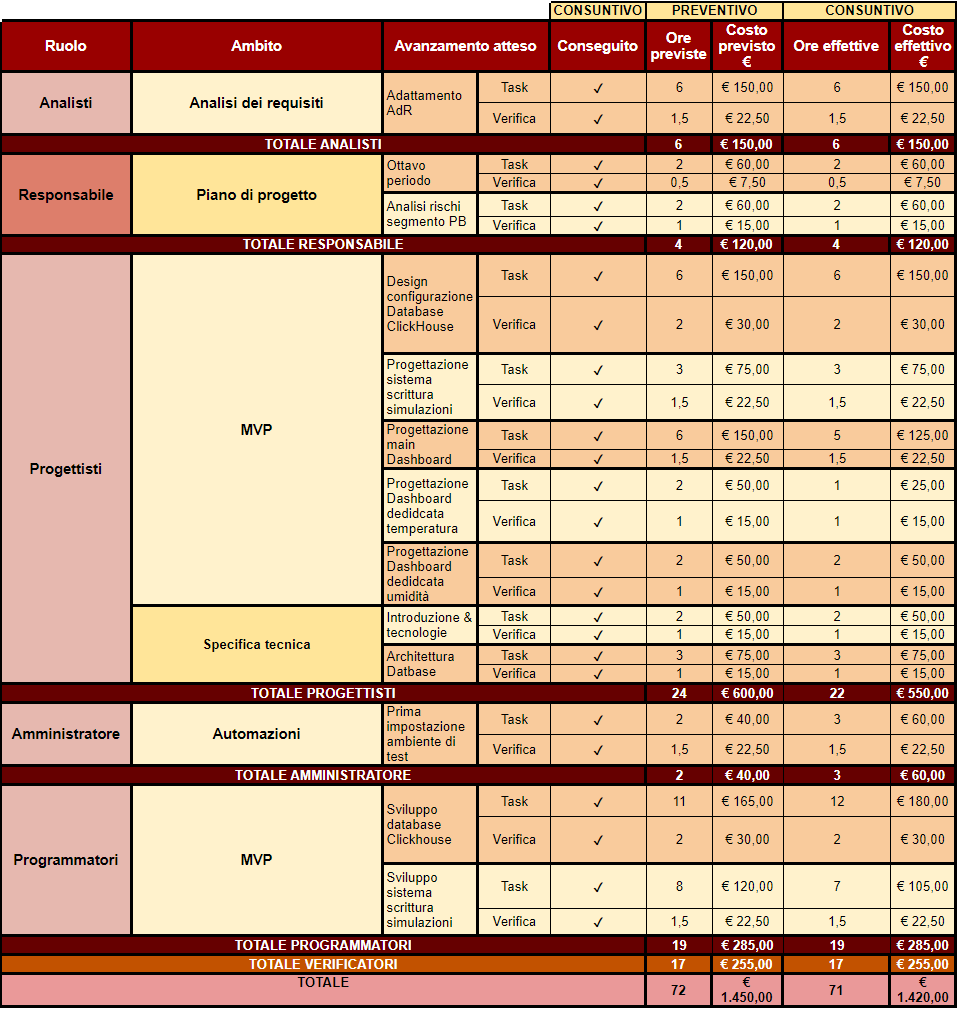
\includegraphics[height=1.1\textwidth]{../Images/periodo8.PNG}
    \caption{Ottavo periodo}
    \label{fig:Ottavo_periodo}
\end{figure}

Al termine dell'ottavo periodo, l'ammontare totale del costo del progetto è \textbf{6012,50\euro} e sono state completate il \textbf{100\%} delle \textit{attività}\textsubscript{\textit{G}} attese.
Il preventivo a finire rimane invariato a \textbf{12425,00\euro} e non risulta necessaria una ripianificazione delle \textit{attività}\textsubscript{\textit{G}} future.
\href{https://github.com/orgs/ByteOps-swe/projects/3/views/1?sortedBy%5Bdirection%5D=asc&sortedBy%5BcolumnId%5D=64182560}{Vai al Diagramma di Gantt.}

\begin{figure}[H]
    \centering
    \begin{minipage}[b]{0.70\textwidth}
        \centering
        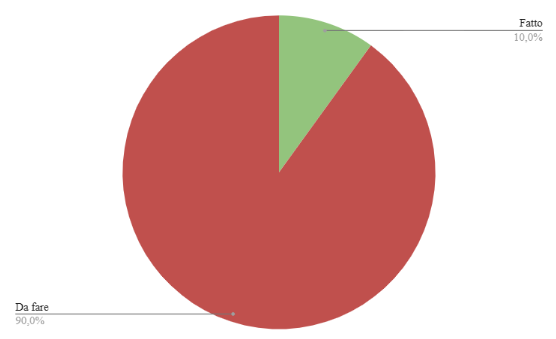
\includegraphics[width=0.7\textwidth]{../Images/avanzamento8Periodo.png}
        \caption{Avanzamento dei lavori RTB - Ottavo periodo}
        \label{fig:Avanzamento_RTB_8}
    \end{minipage}
\end{figure}

\paragraph{Preventivo orario}

\begin{figure}[H] 
    \centering
    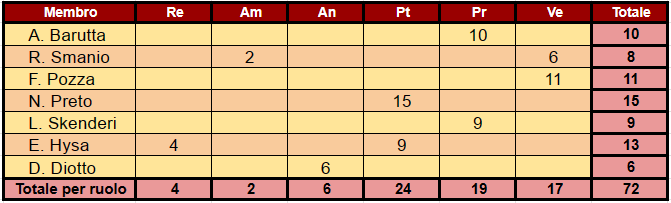
\includegraphics[width=0.9\textwidth]{../Images/preventivoOrario8Periodo.png}
    \caption{Preventivo orario per membro - Ottavo periodo}
    \label{fig:Preventivo_orario_8}
\end{figure}

\begin{figure}[H]
    \centering
    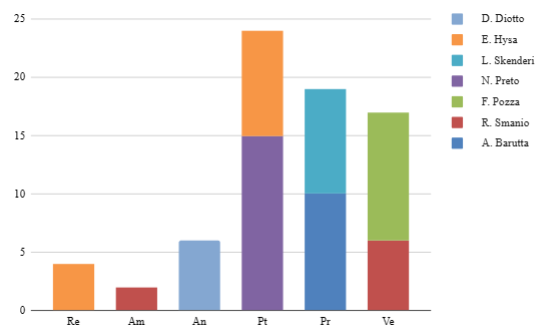
\includegraphics[width=0.6\textwidth]{../Images/preventivoDivisioneRuoli8Periodo.png}
    \caption{Istogramma preventivo della ripartizione oraria dei ruoli - Ottavo periodo}
    \label{fig:Preventivo_ripartizione_oraria_8}
\end{figure}

\paragraph{Consuntivo orario}

\begin{figure}[H]
    \centering
    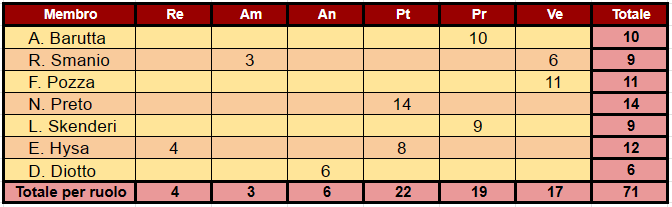
\includegraphics[width=0.9\textwidth]{../Images/consuntivoOrario8Periodo.png}
    \caption{Consuntivo orario per membro - Ottavo periodo}
    \label{fig:Constuntivo_orario_8}
\end{figure}

\begin{figure}[H]
    \centering
    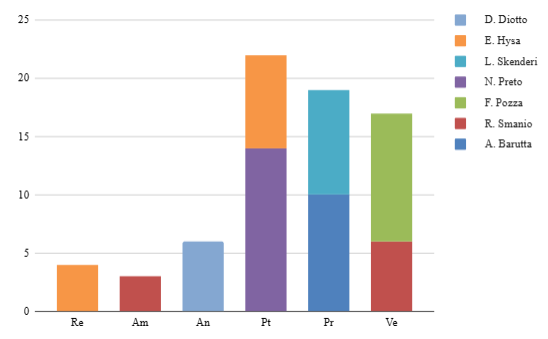
\includegraphics[width=0.6\textwidth]{../Images/consuntivoDivisioneRuoli8Periodo.png}
    \caption{Istogramma consuntivo della ripartizione oraria dei ruoli - Ottavo periodo}
    \label{fig:Consuntivo_ripartizione_oraria_8}
\end{figure}

%---------------------NONO PERIODO---------------------------------------

\subsubsection{Nono periodo  23/02/2024 - 01/03/2024}

\paragraph{Considerazioni}
Durante il nono periodo, sono stati dedicati notevoli risorse alle attività di progettazione, sviluppo e testing relative al Minimum Viable Product (MVP). I progettisti e gli sviluppatori hanno completato le attività di progettazione e sviluppo delle dashboard in Grafana. Questo ha portato alla realizzazione di una dashboard principale, concepita per offrire una visione d'insieme dello stato di salute della città, e una dashboard secondaria, pensata per consentire un'analisi dettagliata delle misurazioni mediante l'applicazione di filtri personalizzati. \\
In seguito al completamento delle dashboard, è stata avviata la redazione del \textit{Manuale Utente}. È importante notare che le sezioni del \textit{Manuale Utente} redatte nell'attuale periodo non sono state ancora verificate, ma tale verifica è stata pianificata per il periodo successivo, garantendo così una quantità adeguata di materiale da esaminare.
Progettisti e programmatori, oltre alla realizzazione delle dashboard, hanno portato a termine la progettazione e lo sviluppo del database e si sono inoltre dedicati all'implementazione della funzionalità di calcolo del punteggio di salute utilizzando la libreria Faust. \\
Per quanto riguarda il documento "\textit{Specifica Tecnica}", sono state completate le sezioni "Introduzione" e "Scelte Tecnologiche" ed è stata avviata la redazione della sezione relativa all'architettura del database. \\
Nell'attuale periodo, l'amministratore si è dedicato alla modifica della struttura della repository, in risposta alle osservazioni ricevute dal Prof. Vardanega durante la revisione RTB. Grazie a quest'intervento, la repository è stata resa più semplice e intuitiva, soddisfacendo così le richieste di miglioramento. \\
Parallelamente allo sviluppo delle componenti principali del sistema, sono stati avviati i test, con particolare attenzione allo sviluppo dei test di unità per i simulatori dei sensori e dei test di integrazione tra Python e Kafka e tra Python e Clickhouse.

\paragraph{Gestione dei rischi} \todo{completa}

\begin{itemize}
    \item \textbf{Rischi attesi e verificati:}
    \begin{itemize}
        \item \textbf{RO-2A-4} - Inesperienza nell'\textit{attività}\textsubscript{\textit{G}} di testing (\textit{\ref{sec:inexpAttività}})   \todo{guardando anche i verbali scrivi qualcosa di relativo alle difficoltà incontrate}
        \begin{itemize}
            \item \textbf{Esito della mitigazione}:
            \item \textbf{Impatto}:
        \end{itemize}
    \end{itemize}
\item \textbf{Rischi attesi ma non verificati:}
    \begin{itemize}
        \item \textbf{RO-2A-4} - Inesperienza nell'\textit{attività}\textsubscript{\textit{G}} di progettazione (\textit{\ref{sec:inexpAttività}}) \todo{qui potrei scrivere che in seguito allo sviluppo di minimal working example realizzati nel precedente periodo non si sono verificate difficoltà nella progettazione}
    \end{itemize} 
\item \textbf{Rischi non attesi ma verificati:}
    \begin{itemize}
        \item Nessuno
    \end{itemize}
\end{itemize}


\paragraph{Definizione ruoli}
Per le \textit{attività}\textsubscript{\textit{G}} registrate nei costi, sono stati assegnati i seguenti ruoli: 

\begin{table}[H]
    \centering
    \begin{tabular}{|L{4cm}|L{2cm}|}
        \hline
        \textbf{Ruolo} & \textbf{Persona} \\
        \hline
        \hline
        Responsabile (Re)   & L. Skenderi \\
        \hline
        Amministratore (Am) & F. Pozza \\
        \hline
        Analisti (An)       & L. Skenderi \\
        \hline
        Verificatore (Ve)   & E. Hysa \\
                            & N. Preto \\
                            & A. Barutta \\
                            & L.Skenderi \\   
        \hline
        Programmatori (Pr)  & R. Smanio \\
                            & D. Diotto \\
        \hline
        Progettista (Pt)    & A. Barutta \\
                            & F. Pozza \\
        \hline
    \end{tabular}
    \caption{Tabella dei ruoli assegnati - Nono periodo}
    \label{tab:Ruoli_persone_9}
\end{table}

\paragraph{Pianificazione attività divise per ruoli con consuntivo e preventivo orario e dei costi}

\vspace{0.4cm}

\begin{figure}[H]
    \centering
    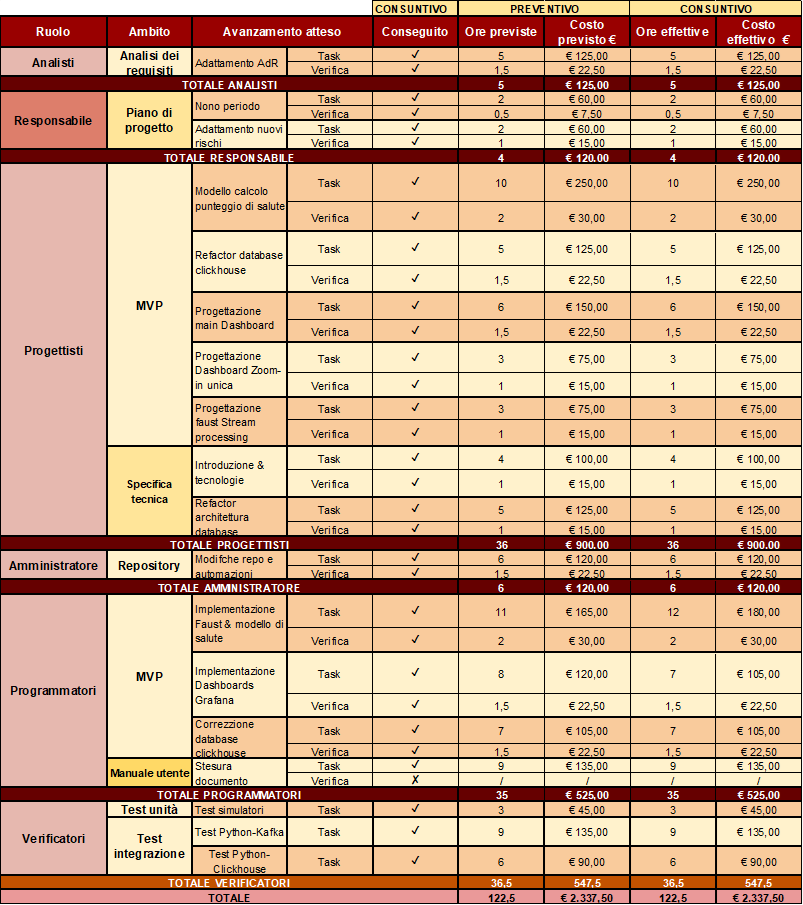
\includegraphics[height=1.1\textwidth]{../Images/periodo9.PNG}
    \caption{Nono periodo}
    \label{fig:Nono_periodo}
\end{figure}

Al termine del nono periodo, l'ammontare totale del costo del progetto è \textcolor{red}{\textbf{XXX \euro}}\todo{inserisci} e sono state completate il \textbf{100\%} delle \textit{attività}\textsubscript{\textit{G}} attese.
Il preventivo a finire rimane invariato a \textbf{12425,00\euro} e non risulta necessaria una ripianificazione delle \textit{attività}\textsubscript{\textit{G}} future.
\href{https://github.com/orgs/ByteOps-swe/projects/3/views/1?sortedBy%5Bdirection%5D=asc&sortedBy%5BcolumnId%5D=64182560}{Vai al Diagramma di Gantt.}

\begin{figure}[H]
    \centering
    \begin{minipage}[b]{0.70\textwidth}
        \centering
        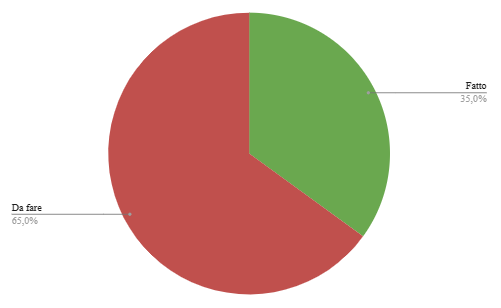
\includegraphics[width=0.7\textwidth]{../Images/avanzamento9Periodo.png}
        \caption{Avanzamento dei lavori RTB - Nono periodo}
        \label{fig:Avanzamento_RTB_9}
    \end{minipage}
\end{figure}

\paragraph{Preventivo orario}

\begin{figure}[H] 
    \centering
    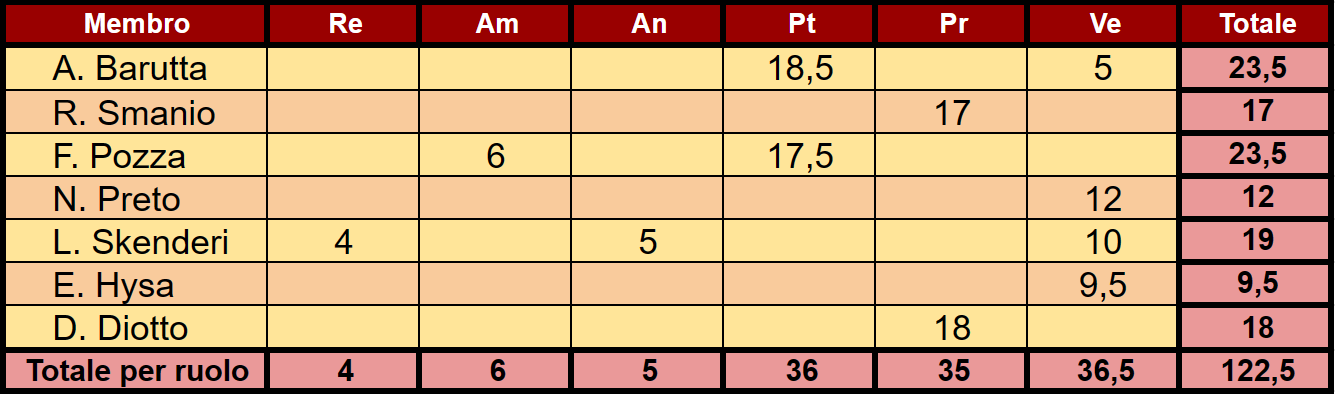
\includegraphics[width=0.9\textwidth]{../Images/preventivoOrario9Periodo.png}
    \caption{Preventivo orario per membro - Nono periodo}
    \label{fig:Preventivo_orario_9}
\end{figure}

\begin{figure}[H]
    \centering
    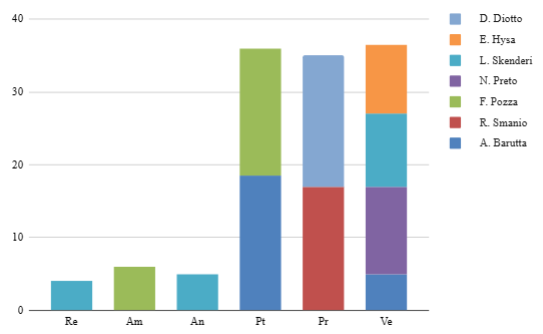
\includegraphics[width=0.6\textwidth]{../Images/preventivoDivisioneRuoli9Periodo.png}
    \caption{Istogramma preventivo della ripartizione oraria dei ruoli - Nono periodo}
    \label{fig:Preventivo_ripartizione_oraria_9}
\end{figure}

\paragraph{Consuntivo orario}

\begin{figure}[H]
    \centering
    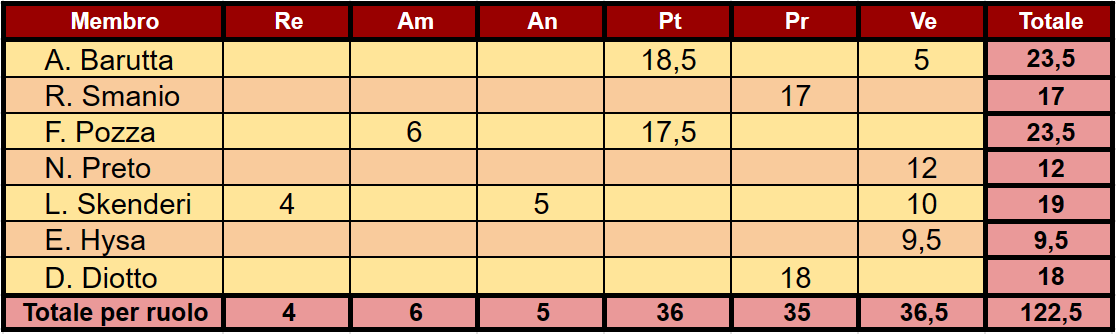
\includegraphics[width=0.9\textwidth]{../Images/consuntivoOrario9Periodo.png}
    \caption{Consuntivo orario per membro - Nono periodo}
    \label{fig:Constuntivo_orario_9}
\end{figure}

\begin{figure}[H]
    \centering
    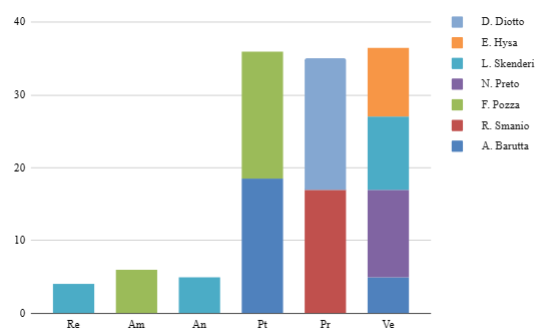
\includegraphics[width=0.6\textwidth]{../Images/consuntivoDivisioneRuoli9Periodo.png}
    \caption{Istogramma consuntivo della ripartizione oraria dei ruoli - Nono periodo}
    \label{fig:Consuntivo_ripartizione_oraria_9}
\end{figure}